
\section{Introduction}

The Lossy Compression WG was formed in response to \jira{RFC-325} with its charter
being \citeds{LDM-582}.  The purpose was to investigate whether some pipeline products
(images) might be saved after applying a lossy compression algorithm without significantly
degrading their suitability for many scientific investigations.  The main reason 
for such a change would be to provide community access to some products without 
requiring on-the-fly reprocessing from the raw data.

In \jira{RFC-325} it was recognized that user 
experience will be unacceptably impacted by the long latency required to 
access the LSST data from tape media. Unfortunately, preliminary analysis
indicated that retaining all processed images on disk would be too costly 
and therefore not feasible, unless lossy compression is applied. The same
analysis indicated that storing all raw data on disk (w/o lossy compression)
is feasible.

The LSST has traditionally avoided lossy compression for any of its image 
data products (including the large co-added images as well as templates 
retained for each data release). Anecdotal experience from the Dark Energy 
Survey (DES) and other surveys (e.g. HSC) indicates that lossy compression 
can be applied, without loss of scientific fidelity.  If this is the case, 
the reduced disk space needs may enable LSST to retain on low-latency media 
more data that we otherwise would (rather than regenerate or pull from tape). 


\section{Methodology}

This investigation is not meant to address the specific file format(s) that might be
used to store LSST data (e.g.; FITS vs. HDF5).  The tests that have been made were performed
using images stored using FITS, mainly because the changes necessary could be used within 
the current LSST pipeline testing infrastructure.  The specific images used were a set of
HSC data that formed a modest depth tract on which pipeline regression testing was already
being routinely performed in the development of the LSST pipelines.  For this test set there
were 33 images/CCDs, from 11 visit/exposures, at two bands (HSC-R, HSC-I).  Included among
these images are a 4 images near the edge of the HSC focal-plane, where vignetting causes
a portion of the detector unusable for science.  These regions are masked and present very 
different noise characteristics but are useful because they show some caveats that must be
considered when applying compression.

A change has been injected into the pipeline that allows for a quantization to be applied
to the science (and weight) images that are traditionally stored as floats.  Formally,
the quantization factor, q, determines the number of samples/subdivisions of some set
number, in this case the standard-deviation of the image pixels that do not contain a 
detected source.  For a FITS image this is expressed as a scale factor (BSCALE) and the image 
pixel values are converted to the nearest integer multiple of this factor.  We then use existing
loss-less compression algorithms to compress the integer representation of the image
to achieve a compressed image.  Our tests varied the factor q from 4 to 128 (stepping by 
factors of 2).

Metrics are then obtained to understand the impact and efficacy of compression.  Broadly, 
these fall into three categories:
\begin{enumerate}
\item {\bf Image Compression benchmarks:} to measure the changes at the pixel level.  These
include: percent increase in noise/RMS, median difference, and number of pixels that change
by more than the quantization level (to catch cases where the integer representation is not 
able to capture the full dynamic range of the original images).

\item {\bf Catalog/Measurement benchmarks:} to measure the change of aggregate quantities
of interest for scientists using the images for scientific measurements.  The current
benchmarks being measured are source position, flux, and shape along with their associated
uncertainties.

\item {\bf Compression algorithm benchmarks:} to measure the compression factor achieved, along with
algorithm execution times for compression and decompression.
\end{enumerate}
In addition a second round of image and catalog benchmarks can also be obtained to assess
the changes that might be expected when compressed products are combined to form stacked
images from which astronomical source measurements are also obtained.


\section{Results}

\subsection{Image Compression Benchmarks}

At the image level, independent measurements of the noise in the original science 
and weight images (I$_{0}$, W$_{0}$) and the quantized versions (I$_{\rm q}$, W$_{\rm q}$) are made.
The algorithms used are independent of those that performed the estimates used to set the quantization.
In most cases we consider only pixels with FLAG=0 or FLAG=32 (which indicates the presence of a source)
as heavily masked regions often have values (particularly in the weight image) that can exceed the 
range accessible in the quantized images.  Figure~\ref{pixel_dist} shows the distributions of pixels
values for the science and weight planes from two images typical of those in the test set.

\begin{figure}
\centering
  \begin{minipage}{.475\textwidth}
    \centering
    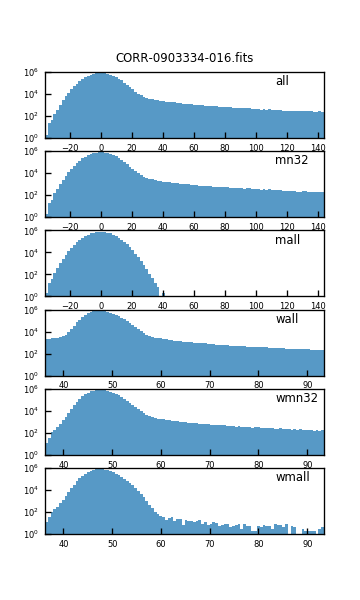
\includegraphics[width=1.0\textwidth]{figure/imgdist_CORR-0903334-016.fits.png}
%    \label{fig:sub1}
  \end{minipage}
  \begin{minipage}{.475\textwidth}
    \centering
    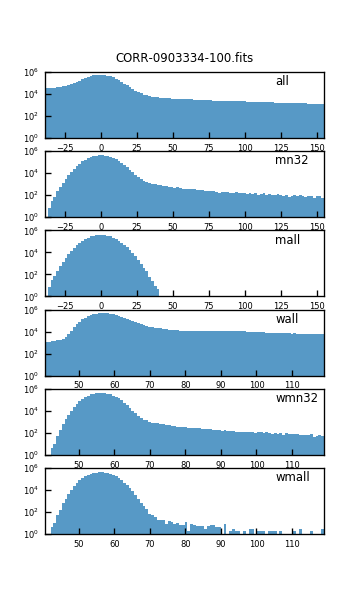
\includegraphics[width=1.0\textwidth]{figure/imgdist_CORR-0903334-100.fits.png}
%   \label{fig:sub2}
  \end{minipage}
\caption{Histograms showing distribution of pixel values for two images in the set. (left) panels show 
distributions for a normal image, while (right) panels show the distributions for an image near the edge 
of the focal plane with heavy masking.  (top) to (bottom) the panels show: all science plane pixels (all), 
all science pixels with MASK=0 or 32 (mn23), and all unmasked pixels (mall), followed by similar
distributions for the weight plane (wall, wmn32, and wmall).  Note the "mall" and "wmall" are roughly
the distribution that was used to estimate the quantization level.}
\label{pixel_dist}
\end{figure}

A base level check is made to that examines the difference between the quantized and unquantized version
of an image (${\rm I}_{\rm diff} = {\rm I}_{\rm q}-{\rm I}_{\rm 0}$).  First the mean  
($\bar{{\rm I}_{\rm diff}}$) and RMS ($\sigma_{{\rm I}_{\rm diff}}$) are computed to show that no
systematic offset occurs and that the noise in the difference is indeed less than the scale factor.
We then also search for pixels where the difference exceeds the quantization level.  For most images
this latter value is identically zero but in a small number of cases the pixels in a bright object
will exceed the range available in the quantized image (i.e. the integer representation has insufficient
cardinality to track the dynamic range in the image).  If flagged pixels are included, then are typically
more pixels that exceed this range and in the worst cases (e.g. images from CCDs that are vignetted) a
large fraction of the weight pixels cannot be tracked.
{\bf More needed to quantitatively describe these?}

We then measure the standard deviation (RMS) in each science and weight image ($\sigma_{{\rm I}_{\rm q}}$ 
and $\sigma_{{\rm W}_{q}}$ respectively) to understand the fractional increase in the image noise
from the quantization ( $\sigma_{\rm grow} = \sqrt(\sigma_{{\rm I}_{q}}^2 - \sigma_{{\rm I}_{0}}^2 )$.  
Figures~\ref{image_difference} and \ref{weight_difference} show histograms of these metrics based
on the images in this test set.  The left panels show the residual noise as measured from the difference
between the unquantized and quantized images.  The right panels show the fractional additive noise 
resulting from the quantization.  Note that the number of samples in the histograms for q=64 and 128 
this is because the measurement of the standard deviation is approaching the machine accuracy (i.e. 
$\sigma_{{\rm I}_{q}}$ differs from $\sigma_{{\rm I}_{0}}$ by less than a part in 10$^{6}$).

\begin{figure}
\centering
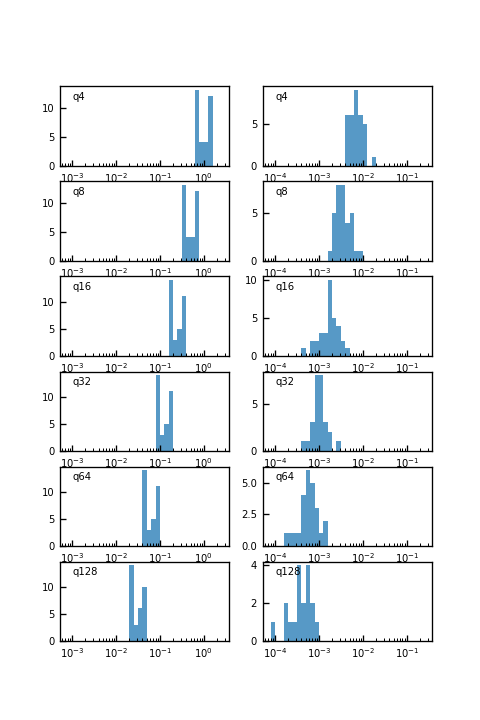
\includegraphics[width=0.75\textwidth]{figure/compression_metric_v2.png}
\caption{Histograms showing image level statistics with respect to the original compressed image.
(left panels) are histograms showing the RMS of the difference between the compressed and original image. 
(right panels) are histograms of the fractional increase in the noise with respect to the original image.}
\label{image_difference}
\end{figure}


\begin{figure}
\centering
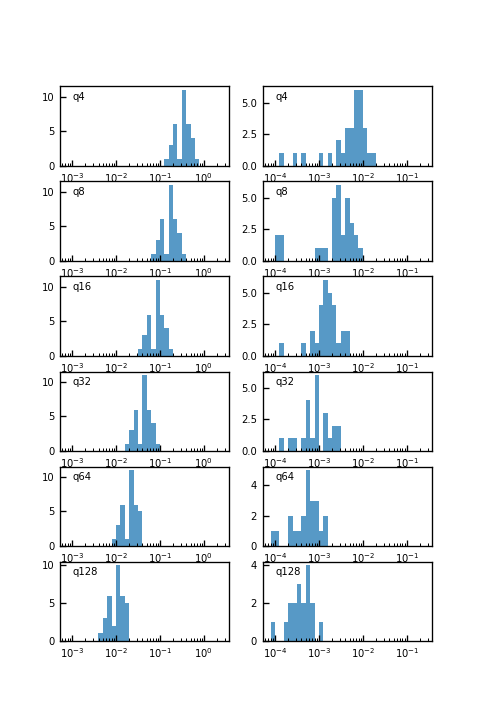
\includegraphics[width=0.75\textwidth]{figure/compression_metric_v2w.png}
\caption{Similar to Figure~\ref{image_difference} but for the weight image.}
\label{weight_difference}
\end{figure}


\subsection{Aggregate Image Compression Benchmarks}

Beside the individual images, a coadded patch was constructed from the never-compressed and then the quantized data 
products.  While only two coadded images were produced per test run, these can be put through a comparison similar 
to that made for the individual images to get a sense of the down-stream consequences if compressed images were used
to construct coadd images.  The results from those comparisons are summarized in Table~\ref{tab_agg_image}.  One 
difference in how the comparison is performed for the COADDed patch is that flagged pixels are now included.


\begin{table}
\caption{Compression Factor Achieved {\bf THIS IS SIMPLY A COPY/PLACEHOLDER}}
\centering
\begin{tabular}[]{crrrrrrrrr}
\hline
 q        &  gzip & pigz & bzip2 & pbzip2 & lbzip2 & lz4 & lzop & zstd & zstdb  \\
\hline
 q4       &   6.73 &  6.73 &  9.96 &  9.95 &  9.96 &  3.69 &  3.11 &  6.29 &  6.29  \\
 q8       &   5.54 &  5.53 &  8.20 &  8.20 &  8.21 &  3.34 &  2.96 &  5.42 &  5.42  \\
 q16      &   4.69 &  4.69 &  5.41 &  7.01 &  7.03 &  3.11 &  2.82 &  4.82 &  4.82  \\
 q32      &   4.04 &  4.03 &  6.14 &  6.14 &  6.14 &  2.93 &  2.66 &  4.35 &  4.35  \\
 q64      &   3.62 &  3.62 &  5.47 &  5.47 &  5.48 &  2.82 &  2.47 &  3.94 &  3.94  \\
 q128     &   3.38 &  3.37 &  4.88 &  4.88 &  4.88 &  2.66 &  2.32 &  3.56 &  3.57  \\
 vanilla  &   1.71 &  1.71 &  1.80 &  1.80 &  1.80 &  1.50 &  1.49 &  1.72 &  1.72  \\
\hline
\end{tabular}
\label{tab_agg_image}
\end{table}

At the image level, independent measurements of the noise in the original science 
and weight images (I$_{0}$, W$_{0}$) and the quantized versions (I$_{\rm q}$, W$_{\rm q}$) are made.
The algorithms used are independent of those that performed the estimates used to set the quantization.



\subsection{Catalog/Measurement benchmarks}

Here we outline the comparison of measurements made on individual ccd-visit images with and without 
lossy compression applied.  Currently four types of measurements are considered: aperture photometry, 
PSF photometry, centroids, and shapes.  In each case the comparison is made by using forced photometry
based on the COADD catalogs from the {\it ci\_hsc} pipeline applied to the never-quantized and quantized
images and then performing and astrometric match between the never-compressed catalog and those from the
catalogs from the quantized images.  Note a generous match radius of 2\arcsec is used and the nearest match
is considered to measurements of the same object.  

Figures~\ref{plot_app_flux} show comparisons for flux measurements for aperture photometry 
using a 6 pixel radius circular aperture and Figure~\ref{plot_psf_flux} for PSF fitting, respectively.
In each plot, the top two panels set show (first) the total number of objects 
per flux bin and then a plot showing the flux uncertainty as a function of flux from the never compressed image.  
Beneath these are plotted the difference between the measurements from the quantized images and the never-quantized 
images with subsequent plots using an increasing level of quantization.  These differnce plots are shown in units of
$\sigma_{\rm F_0}$.  Also plotted are histograms showing the diffence level that encompasses 50, 75, 90, and 99\% of the 
measurements as a function of flux bin.

\begin{figure}
\centering
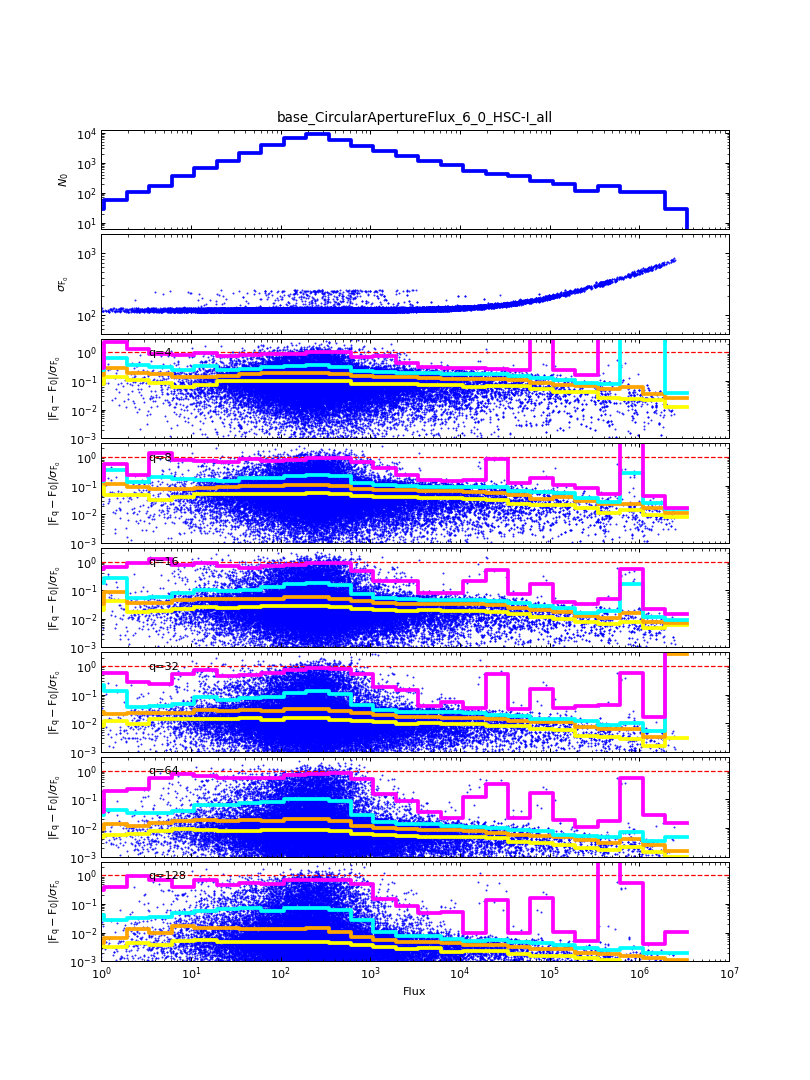
\includegraphics[width=0.75\textwidth]{figure/rplot_all_base_CircularApertureFlux_6_0_HSC-I.png}
\caption{Comparison of aperture photometry measurements (from a 6 pixel radius aperture) resulting from forced photometry 
on individual images with and without quantization/compression.
The top panel shows the distrubution of objects as a function of their flux measured in the original image(s).  The second show 
measure uncertainties for those flux measurements.  The panels below show the difference between the flux measurements made on the
unquantized and quantized images divided by the uncertainty in the quantized images (in units of $\sigma_{\rm F_0}$.  A dashed horizontal 
red line shows the 1$\sigma$ difference level for reference.  Lower panels are employed systematically higher quantization factors on the
images.  The histograms in each panel show the difference level at which 50, 75, 90 and 90\% of the objects are found.}
\label{plot_app_flux}
\end{figure}

\begin{figure}
\centering
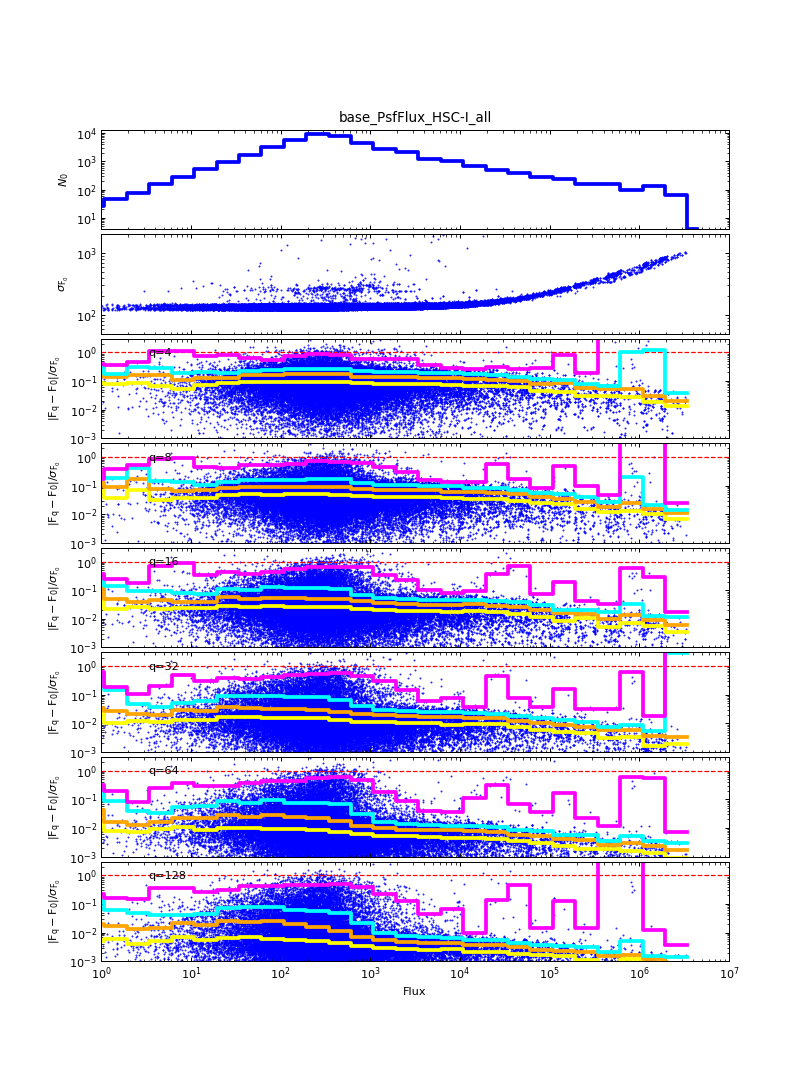
\includegraphics[width=0.75\textwidth]{figure/rplot_all_base_PsfFlux_HSC-I.png}
\caption{Same as Figure~\ref{plot_app_flux} but for PSF fitting photometry.}
\label{plot_psf_flux}
\end{figure}


Figure~\ref{plot_cen} shows comparisons of centroid and Figure~\ref{plot_shape} show shape measurements as a function of signal to noise 
(in the unquantized image).  For the centroids the units are in pixels offset between the measurement made on the 
never-quantized and quantized images, $X_q-X_0 = \sqrt{ (x_q-x_0)^2 + (y_q-y_0)^2}$.  
For the shapes we have defined the parameter $S=(I_{xx} I_{yy} - I_{xy}^2)^{1/4}$ (akin to a radius) 
where the uncertainty can be expressed as $\sigma_S^2 = (\frac{\partial S}{\partial I_{xx}})^2 \sigma_{I_{xx}}^2 + 
(\frac{\partial S}{\partial I_{yy}})^2 \sigma_{I_{yy}}^2 + (\frac{\partial S}{\partial I_{xy}})^2 \sigma_{I_{xy}}^2$.

\begin{figure}
\centering
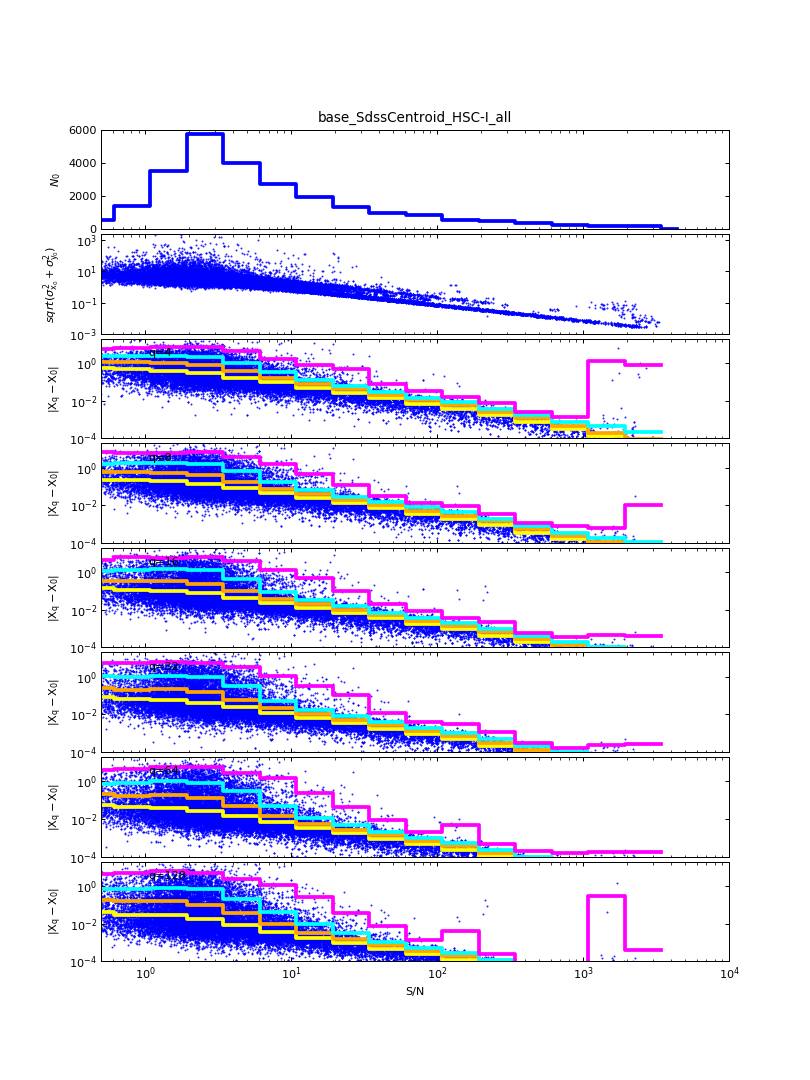
\includegraphics[width=0.75\textwidth]{figure/rplot_all_base_SdssCentroid_HSC-I.png}
\caption{Similar to Figures~\ref{plot_app_flux}\&\ref{plot_psf_flux} but for centroid measurements as function of the signal-to-noise ratio
of the unquantized measurements.  The differences in the lower panels are in units of pixel offset.}
\label{plot_cen}
\end{figure}

\begin{figure}
\centering
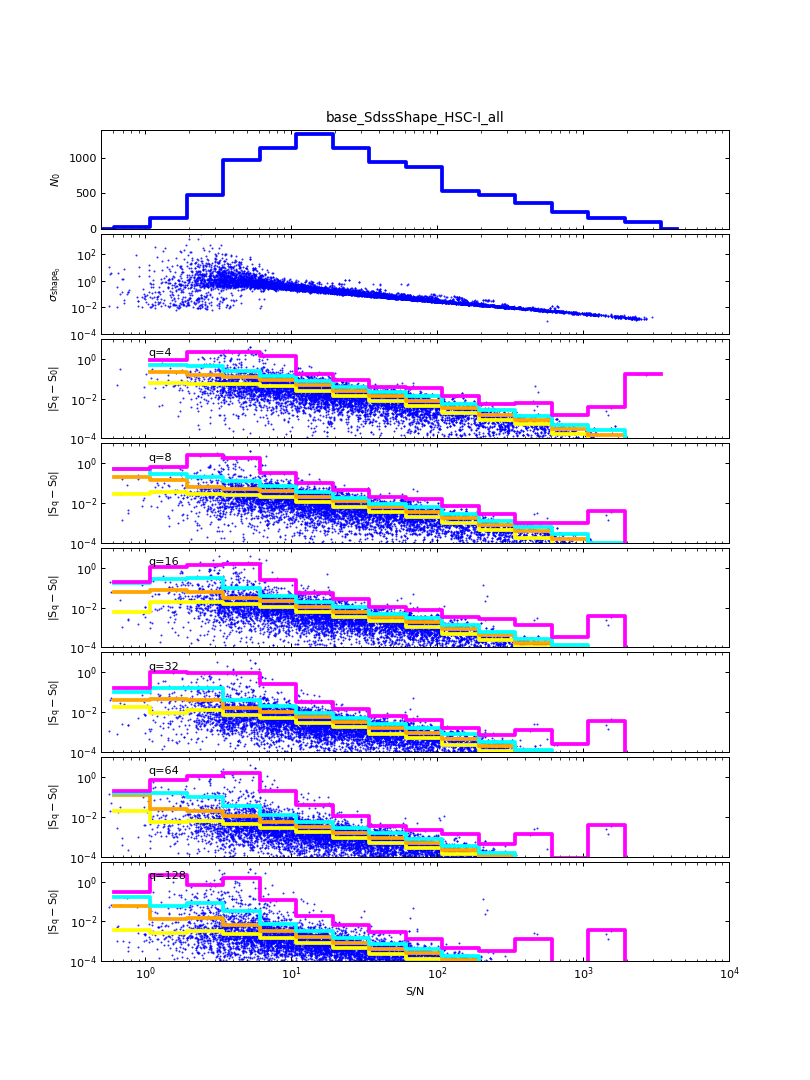
\includegraphics[width=0.75\textwidth]{figure/rplot_all_base_SdssShape_HSC-I.png}
\caption{Similar to Figure~\ref{plot_cen} but for the SDSS shape measurments.  The comparison is made using the quantity S which is equivalent to
a size/radius.}
\label{plot_shape}
\end{figure}




\subsection{Catalog/Measurement from COADD images constructed from quantized PVI images}


\begin{figure}
\centering
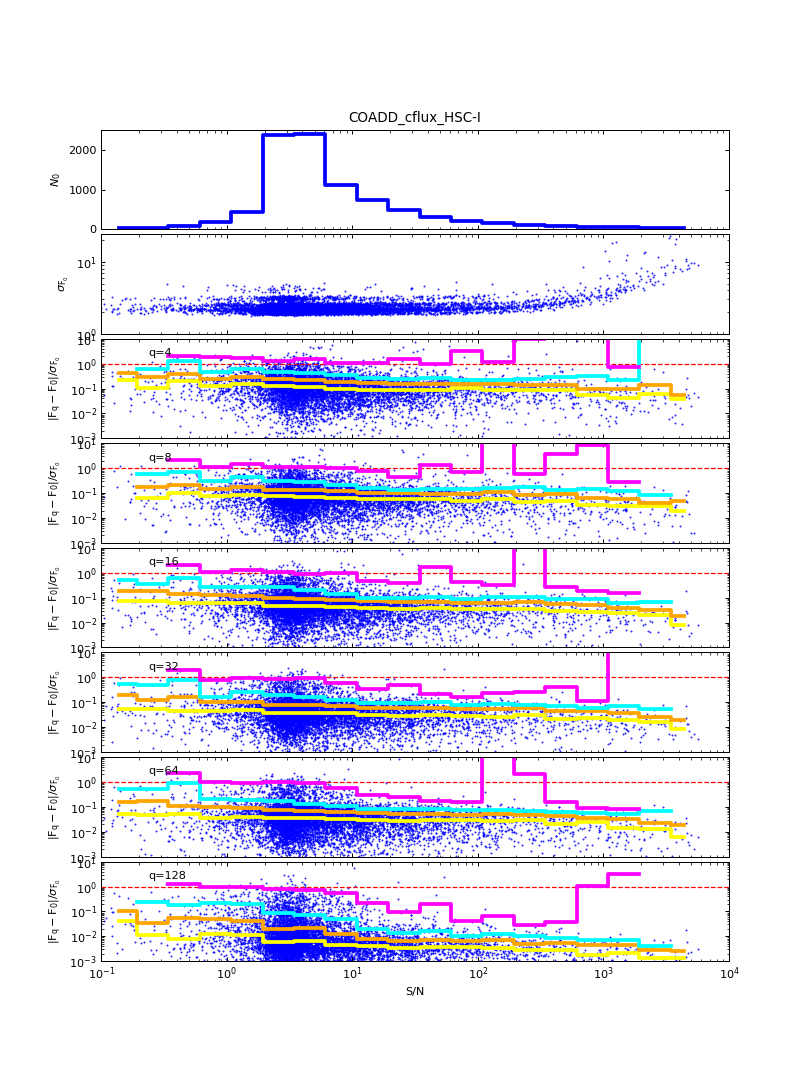
\includegraphics[width=0.75\textwidth]{figure/plot_coadd_cflux_HSC-I.png}
\caption{Similar to Figure~\ref{plot_app_flux} but comparing measurements made on COADD images constructured from 
never quantized and quantized images.}
\label{coadd_app_flux}
\end{figure}

\begin{figure}
\centering
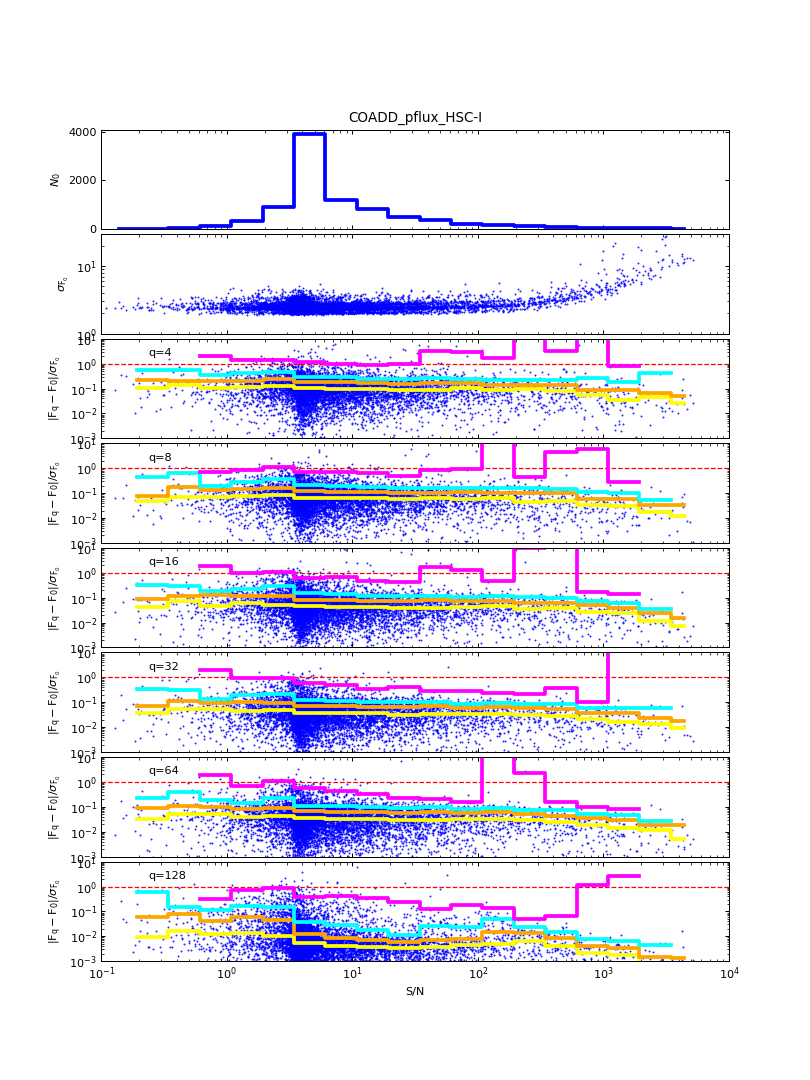
\includegraphics[width=0.75\textwidth]{figure/plot_coadd_pflux_HSC-I.png}
\caption{Same as Figure~\ref{coadd_app_flux} but for PSF fitting photometry.}
\label{coadd_psf_flux}
\end{figure}


\begin{figure}
\centering
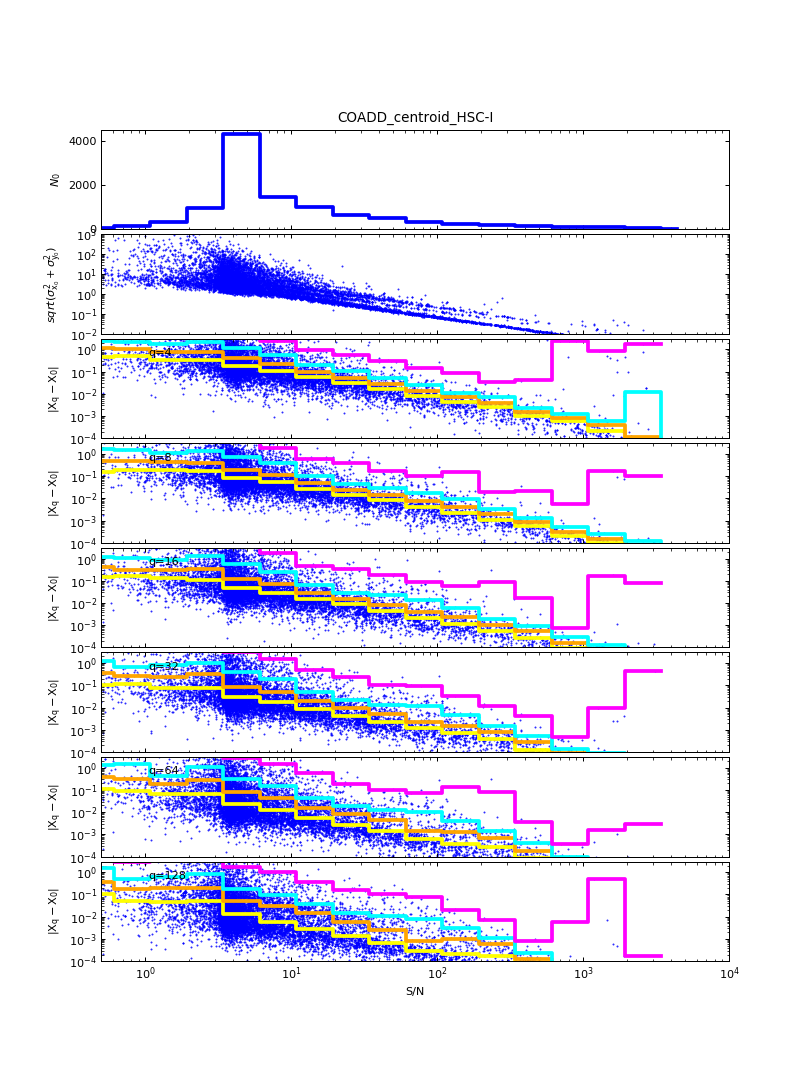
\includegraphics[width=0.75\textwidth]{figure/plot_coadd_centroid_HSC-I.png}
\caption{Similar to Figures~\ref{plot_app_flux}\&\ref{plot_psf_flux} but for centroid measurements as function of the signal-to-noise ratio
of the unquantized measurements.  The differences in the lower panels are in units of pixel offset.}
\label{coadd_cen}
\end{figure}

\begin{figure}
\centering
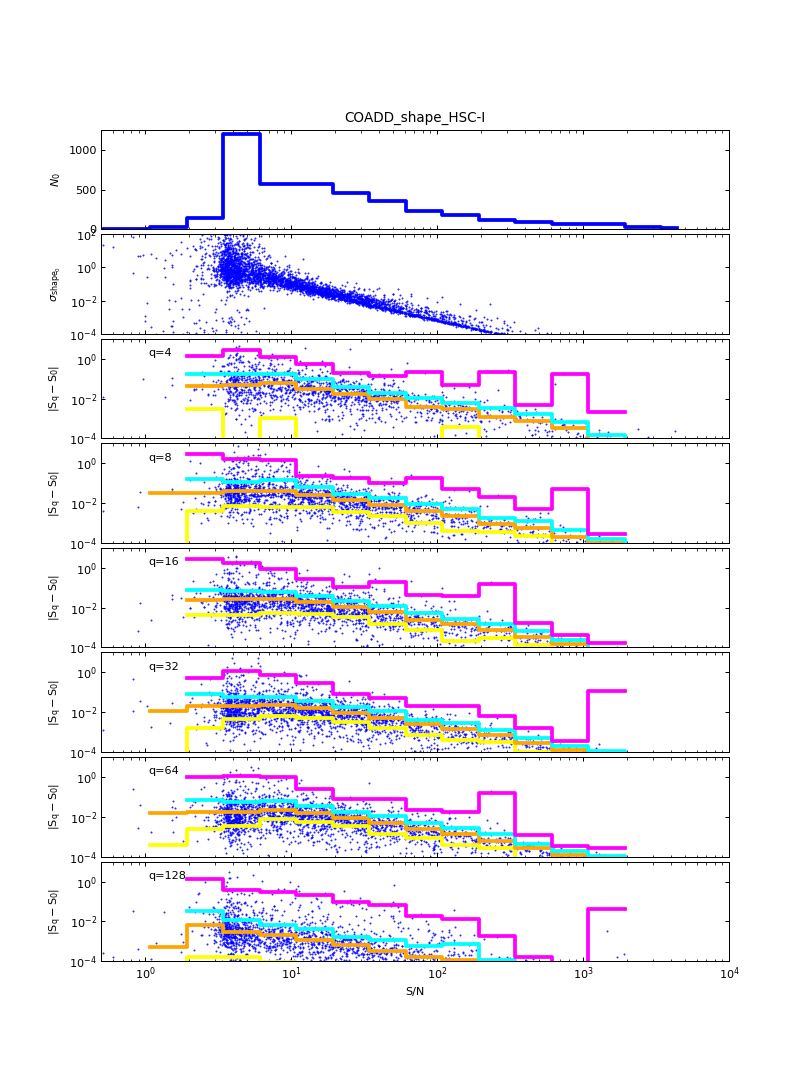
\includegraphics[width=0.75\textwidth]{figure/plot_coadd_shape_HSC-I.png}
\caption{Similar to Figure~\ref{plot_cen} but for the SDSS shape measurments.  The comparison is made using the quantity S which is equivalent to
a size/radius.}
\label{coadd_shape}
\end{figure}






\subsection{Compression Algorithm benchmarks}

We have applied a variety of existing compression algorithms to the quantized images from this study to 
obtain benchmarks of their efficacy.  The values reported reflect those algorithms' performance when
running under OS X 10.13.2 (macOS High Sierra) on a MacBook Pro with quad 2.9 GHz processors.  A ramdisk
was used for storage to minimize the impact of I/O operations within the test.  

A range of existing algorithms have been benchmarked, including a number which use threading to achieve 
greater speed.  The algorithms considered were:
\begin{enumerate}
\item {\bf gzip:} the standard GNU implementation of Lempel-Ziv (LZ77).
\item {\bf pigz:} a threaded version of gzip.
\item {\bf bzip2:} an implementation of Burrows-Wheeler block sorting (offers the possibility of recovery of undamage block).
\item {\bf pbzip2:} a threaded/parallel implementation of bzip2.
\item {\bf lbzip2:} another threaded/parallel implementation of bzip2.
\item {\bf lz4:} a "typically faster" implementation of LZ77 (favoring speed over compression ratio). Pushing to higher compression ratios significantly degrades performance.
\item {\bf lzop:} a separate implementation that trades a small hit in compression time for an improvement in decompression.  The performance trade is not apparent at the file size being used in these tests.
\item {\bf zstd:} Also based on the LZ77 family and includes a parallel implementation.  In addition this
algorithm has implementations/bindings over a wide variety of languages (including Python).  
The usage of a pre-computed dictionary may offer improvement in speed/compression factor but 
rigorous testing was not possible for this small set (performance was identical to the untrained
algorithm if the full set was used both to train and then obtain benchmarks).
\item {\bf xz:} 
\end{enumerate}

The results from benchmark tests are summarized in Tables~\ref{compress_factor}-\ref{timing_decompress}, 
showing compression factor, time to compress per file, and time to decompress per file, respectively.
These times do not include the time to necessary to obtain and apply scale factor used in the quantization.  Furthermore, the set of files being compressed are nearly identical (98 Mb) and therefore do not provide 
any information about algorithmic performance with respect to file size.  When a parallel implementation
was available the threading was set to use 4 cores.


\begin{table}
\caption{Compression Factor Achieved}
\centering
\begin{tabular}[]{crrrrrrrrr}
\hline
 q        &  gzip & pigz & bzip2 & pbzip2 & lbzip2 & lz4 & lzop & zstd & zstdb  \\
\hline
 q4       &   6.73 &  6.73 &  9.96 &  9.95 &  9.96 &  3.69 &  3.11 &  6.29 &  6.29  \\
 q8       &   5.54 &  5.53 &  8.20 &  8.20 &  8.21 &  3.34 &  2.96 &  5.42 &  5.42  \\
 q16      &   4.69 &  4.69 &  5.41 &  7.01 &  7.03 &  3.11 &  2.82 &  4.82 &  4.82  \\
 q32      &   4.04 &  4.03 &  6.14 &  6.14 &  6.14 &  2.93 &  2.66 &  4.35 &  4.35  \\
 q64      &   3.62 &  3.62 &  5.47 &  5.47 &  5.48 &  2.82 &  2.47 &  3.94 &  3.94  \\
 q128     &   3.38 &  3.37 &  4.88 &  4.88 &  4.88 &  2.66 &  2.32 &  3.56 &  3.57  \\
 vanilla  &   1.71 &  1.71 &  1.80 &  1.80 &  1.80 &  1.50 &  1.49 &  1.72 &  1.72  \\
\hline
\end{tabular}
\label{compress_factor}
\end{table}


\begin{table}
\caption{Time to Compress per File}
\centering
\begin{tabular}[]{crrrrrrrrr}
\hline
 q        &  gzip & pigz & bzip2 & pbzip2 & lbzip2 & lz4 & lzop & zstd & zstdb  \\
\hline
 q4       &    4.45 &   1.18 &   5.00 &   1.42 &   0.85 &   0.21 &   0.24 &   0.36 &   0.12  \\
 q8       &    6.06 &   1.64 &   4.91 &   1.39 &   0.82 &   0.21 &   0.24 &   0.42 &   0.15  \\
 q16      &    8.27 &   2.24 &   4.33 &   1.39 &   0.82 &   0.27 &   0.27 &   0.55 &   0.18  \\
 q32      &   10.30 &   2.76 &   5.27 &   1.42 &   0.79 &   0.24 &   0.27 &   0.58 &   0.21  \\
 q64      &   11.79 &   3.00 &   5.39 &   1.52 &   0.88 &   0.24 &   0.30 &   0.61 &   0.24  \\
 q128     &   12.76 &   3.21 &   5.91 &   1.61 &   0.94 &   0.27 &   0.30 &   0.67 &   0.21  \\
 vanilla  &    3.36 &   0.97 &   8.94 &   2.79 &   1.58 &   0.15 &   0.12 &   0.30 &   0.15  \\
\hline
\end{tabular}
\label{timing_compress}
\end{table}

\begin{table}
\caption{Time so Decompress per File}
\centering
\begin{tabular}[]{crrrrrrrrr}
\hline
 q        &  gzip & pigz & bzip2 & pbzip2 & lbzip2 & lz4 & lzop & zstd & zstdb  \\
\hline
 q4       &    0.21 &   0.24 &   2.30 &   1.21 &   1.27 &   0.15 &   0.18 &   0.27 &   0.24  \\
 q8       &    0.24 &   0.27 &   2.33 &   1.12 &   1.24 &   0.18 &   0.18 &   0.27 &   0.27  \\
 q16      &    0.27 &   0.27 &   2.02 &   1.12 &   1.21 &   0.18 &   0.18 &   0.27 &   0.24  \\
 q32      &    0.30 &   0.30 &   2.42 &   1.24 &   1.24 &   0.15 &   0.18 &   0.27 &   0.24  \\
 q64      &    0.30 &   0.30 &   2.42 &   1.27 &   1.09 &   0.18 &   0.21 &   0.27 &   0.27  \\
 q128     &    0.30 &   0.33 &   2.82 &   1.30 &   1.24 &   0.24 &   0.21 &   0.30 &   0.27  \\
 vanilla  &    0.39 &   0.36 &   4.36 &   1.48 &   1.27 &   0.15 &   0.12 &   0.24 &   0.24  \\
\hline
\end{tabular}
\label{timing_decompress}
\end{table}


\section{Mapping Measurements to SRD?}


\section{Recommendations}

The Working Group will provide a recommendation on the suitability of the implementation
of a lossy compression algorithm of LSST products with a figure of merit that can be 
applied with the LSST Sizing Model (\citedsp{LDM-144}).


\section{WG Membership}

Membership of roughly four people is optimal and should include persons familiar 
with weak-lensing and difference imaging concerns.
The proposed membership is:

\begin{itemize}
    \item Robert Gruendl (NCSA; \textbf{Chair}),
    \item Paul Price (Princeton),
    \item Bob Armstrong (Princeton),
    \item Krzysztof Findeisen (UW; replacing John Parejko),
    \item Sophie Reed (Princeton),
    \item Eric Morganson (DES/NCSA; observer)
    \item Ben Emmons (EPO Tucson; observer)
\end{itemize}

